\documentclass[aspectratio=169,11pt]{beamer}

\usepackage[utf8]{inputenc}
\usepackage[T1]{fontenc}
\usepackage[polish]{babel}
\usepackage{lmodern}
\usepackage{graphicx}
\usepackage{booktabs}
\usepackage{tabularx}
\usepackage{array}
\usepackage{ragged2e}

\definecolor{Ink}{HTML}{22313F}
\definecolor{Slate}{HTML}{5B677A}
\definecolor{SoftGray}{HTML}{F4F6F8}
\definecolor{AccentOrange}{HTML}{FF5A00}
\definecolor{DeepBlue}{HTML}{2D6CDF}
\definecolor{GoodGreen}{HTML}{1B998B}
\definecolor{RiskRed}{HTML}{C44536}

\usetheme{Boadilla}
\usecolortheme{default}
\setbeamertemplate{navigation symbols}{}
\setbeamertemplate{itemize items}[circle]
\setbeamertemplate{enumerate items}[default]

\setbeamercolor{normal text}{fg=Ink,bg=white}
\setbeamercolor{structure}{fg=AccentOrange}
\setbeamercolor{frametitle}{fg=Ink,bg=white}
\setbeamerfont{frametitle}{series=\bfseries,size=\Large}
\setbeamerfont{title}{series=\bfseries,size=\LARGE}
\setbeamerfont{subtitle}{size=\large}
\setbeamercolor{block title}{fg=white,bg=DeepBlue}
\setbeamercolor{block body}{fg=Ink,bg=SoftGray}
\setbeamercolor{exampleblock title}{fg=white,bg=GoodGreen}
\setbeamercolor{exampleblock body}{fg=Ink,bg=SoftGray}
\setbeamercolor{alertblock title}{fg=white,bg=RiskRed}
\setbeamercolor{alertblock body}{fg=Ink,bg=SoftGray}
\setbeamercolor{footline}{fg=Slate,bg=white}

\setbeamertemplate{footline}{
  \leavevmode
  \begin{beamercolorbox}[wd=\paperwidth,ht=2.7ex,dp=1.1ex,leftskip=1em,rightskip=1em]{footline}
    Software Usability Project - Task 2
    \hfill \insertframenumber{} / \inserttotalframenumber
  \end{beamercolorbox}
}

\newcolumntype{Y}{>{\RaggedRight\arraybackslash}X}
\newcommand{\tagline}[1]{\textcolor{Slate}{\small #1}}
\newcommand{\statbox}[3]{
  \begin{beamercolorbox}[wd=\linewidth,rounded=true,sep=0.6em,center]{#1}
    {\Large\bfseries #2}\par
    {\scriptsize #3}
  \end{beamercolorbox}
}
\setbeamercolor{statOrange}{fg=white,bg=AccentOrange}
\setbeamercolor{statBlue}{fg=white,bg=DeepBlue}
\setbeamercolor{statGreen}{fg=white,bg=GoodGreen}
\setbeamercolor{statRed}{fg=white,bg=RiskRed}

\title[Audyt dostępności Allegro]{Audyt dostępności platformy Allegro}
\subtitle{Task 2: ocena dostępności ścieżki zakupowej według WCAG 2.1 AA}
\author{Adrian Szwaczyk \and Juliusz Radziszewski \and Maciej Żuralski \and Sebastian Kwaśniak}
\date{Software Usability Project}

\begin{document}

\begin{frame}[plain]
  \vspace{0.8cm}
  {\color{AccentOrange}\rule{\textwidth}{1.2pt}}
  \vspace{0.8cm}

  {\usebeamerfont{title}\inserttitle\par}
  \vspace{0.35cm}
  {\usebeamerfont{subtitle}\textcolor{Slate}{\insertsubtitle}\par}
  \vspace{0.9cm}

  \begin{columns}[T,totalwidth=\textwidth]
    \column{0.58\textwidth}
      \textbf{Zakres:} desktopowa wersja Allegro w Google Chrome\par
      \vspace{0.2cm}
      \textbf{Cel:} sprawdzenie, czy proces zakupowy jest dostępny dla osób z deficytami wzrokowymi, motorycznymi i poznawczymi.
    \column{0.35\textwidth}
      \raggedleft
      \textcolor{Slate}{\small Adrian Szwaczyk\\Juliusz Radziszewski\\Maciej Żuralski\\Sebastian Kwaśniak}
  \end{columns}

  \vfill
  {\color{AccentOrange}\rule{0.34\textwidth}{3pt}}
\end{frame}

\begin{frame}{Punkt wyjścia}
  \tagline{Task 2 rozszerza wcześniejszą analizę użyteczności o perspektywę dostępności.}

  \vspace{0.35cm}
  \begin{columns}[T,totalwidth=\textwidth]
    \column{0.52\textwidth}
      \begin{block}{Badane oprogramowanie}
        \textbf{Allegro} - marketplace e-commerce analizowany w widoku desktopowym.

        \vspace{0.25cm}
        Badaliśmy ścieżkę kupującego: od wyszukania produktu, przez filtry i stronę oferty, do koszyka oraz wyboru dostawy i płatności.
      \end{block}

    \column{0.42\textwidth}
      \begin{exampleblock}{Zmiana perspektywy}
        \begin{itemize}
          \item \textbf{Task 1:} użyteczność dla okazjonalnych kupujących.
          \item \textbf{Task 2:} dostępność tej samej ścieżki dla osób ze specyficznymi potrzebami.
        \end{itemize}
      \end{exampleblock}
  \end{columns}
\end{frame}

\begin{frame}{Dla kogo badaliśmy dostępność?}
  \begin{columns}[T,totalwidth=\textwidth]
    \column{0.31\textwidth}
      \begin{block}{Deficyty wzrokowe}
        Osoby niewidome i słabowidzące.

        \vspace{0.25cm}
        Kluczowe potrzeby: teksty alternatywne, logiczne nagłówki, dobry kontrast, obsługa czytnika ekranu.
      \end{block}

    \column{0.31\textwidth}
      \begin{block}{Ograniczenia motoryczne}
        Osoby korzystające głównie z klawiatury lub przełączników.

        \vspace{0.25cm}
        Kluczowe potrzeby: pełna obsługa bez myszy, widoczny fokus, brak pułapek klawiaturowych.
      \end{block}

    \column{0.31\textwidth}
      \begin{block}{Trudności poznawcze}
        Osoby z dysleksją lub problemami z koncentracją.

        \vspace{0.25cm}
        Kluczowe potrzeby: proste komunikaty, przewidywalna nawigacja, ograniczony chaos wizualny.
      \end{block}
  \end{columns}
\end{frame}

\begin{frame}{Zakres scenariusza}
  \tagline{Audyt objął tę samą podstawową ścieżkę zakupową, która była analizowana w Task 1.}

  \vspace{0.25cm}
  \begin{columns}[T,totalwidth=\textwidth]
    \column{0.55\textwidth}
      \begin{enumerate}
        \item Strona główna i wyszukanie frazy \textbf{``mysz komputerowa''}.
        \item Lista wyników: filtry Logitech, nowy stan, bezprzewodowa, szara, 40-90 zł.
        \item Dodatkowe filtry: Allegro Smart, InPost, Super Sprzedawca oraz sortowanie po cenie z dostawą.
        \item Strona oferty: nazwa, cena, dostawa, sprzedawca, zwroty.
        \item Koszyk: dostawa do paczkomatu InPost, płatność BLIK, bez finalnego zakupu.
      \end{enumerate}

    \column{0.38\textwidth}
      \begin{alertblock}{Kontrola dodatkowa}
        Kluczowe ekrany sprawdzaliśmy także przy powiększeniu widoku do \textbf{200\%}, aby ocenić czytelność i stabilność układu.
      \end{alertblock}
  \end{columns}
\end{frame}

\begin{frame}{Metodologia}
  \tagline{To był audyt ekspercki dostępności, a nie badanie statystycznie reprezentatywnej próby użytkowników.}

  \vspace{0.35cm}
  \begin{columns}[T,totalwidth=\textwidth]
    \column{0.24\textwidth}
      \statbox{statOrange}{4}{niezależnych audytorów}
    \column{0.24\textwidth}
      \statbox{statBlue}{30}{pytań kontrolnych}
    \column{0.24\textwidth}
      \statbox{statGreen}{120}{ocen cząstkowych}
    \column{0.24\textwidth}
      \statbox{statRed}{WCAG 2.1 AA}{poziom odniesienia}
  \end{columns}

  \vspace{0.55cm}
  \begin{block}{Narzędzia i techniki}
    \begin{itemize}
      \item checklista WCAG 2.1 AA na poziomie podstawowym i średnio-zaawansowanym,
      \item test obsługi klawiaturą oraz widoczności fokusu,
      \item sprawdzenie z czytnikiem ekranu NVDA,
      \item wsparcie automatyczne: WAVE i Axe DevTools.
    \end{itemize}
  \end{block}
\end{frame}

\begin{frame}{Co mierzyliśmy?}
  \begin{columns}[T,totalwidth=\textwidth]
    \column{0.48\textwidth}
      \begin{block}{Struktura i semantyka}
        \begin{itemize}
          \item teksty alternatywne dla grafik,
          \item hierarchia nagłówków,
          \item poprawne etykiety i relacje formularzy,
          \item role, nazwy i wartości kontrolek.
        \end{itemize}
      \end{block}

      \begin{block}{Czytelność wizualna}
        \begin{itemize}
          \item kontrast minimum 4,5:1,
          \item działanie widoku przy powiększeniu 200\%.
        \end{itemize}
      \end{block}

    \column{0.48\textwidth}
      \begin{block}{Obsługa klawiaturą}
        \begin{itemize}
          \item dostępność elementów aktywnych,
          \item brak pułapek klawiaturowych,
          \item logiczna kolejność i widoczność fokusu.
        \end{itemize}
      \end{block}

      \begin{block}{Formularze i kontekst}
        \begin{itemize}
          \item identyfikacja błędów,
          \item jasne instrukcje,
          \item ostrzeżenia przed zmianą kontekstu, np. nową kartą.
        \end{itemize}
      \end{block}
  \end{columns}
\end{frame}

\begin{frame}{Przykłady kryteriów WCAG}
  \tagline{Checklista była oparta na kryteriach WCAG 2.1 AA istotnych dla procesu zakupowego.}

  \vspace{0.25cm}
  \small
  \renewcommand{\arraystretch}{1.18}
  \begin{tabularx}{\textwidth}{>{\bfseries}p{0.16\textwidth} p{0.48\textwidth} Y}
    \toprule
    Kryterium & Co sprawdzaliśmy? & Przykład w Allegro \\
    \midrule
    1.1.1 &
    Treść nietekstowa: czy obrazy mają sensowne opisy alternatywne. &
    grafiki promocyjne i zdjęcia ofert \\
    1.3.1 &
    Informacje i relacje: struktura nagłówków, etykiet i formularzy. &
    opis oferty i pola dostawy \\
    1.4.3 &
    Kontrast: czy tekst ma minimum 4,5:1 względem tła. &
    ceny, dostawa, etykiety filtrów \\
    1.4.5 &
    Obrazy z tekstem: czy ważny tekst nie jest osadzony w grafice. &
    tabele i opisy sprzedawców \\
    2.1.1 / 2.1.2 &
    Klawiatura: czy ścieżka działa bez myszy i bez pułapek. &
    popupy, galerie i filtry \\
    2.4.4 &
    Cel łącza: czy użytkownik wie, że link otworzy nową kartę. &
    linki w stopce strony \\
    \bottomrule
  \end{tabularx}
\end{frame}

\begin{frame}{Wykonanie badania}
  \tagline{Każdy audytor oceniał tę samą ścieżkę samodzielnie, a następnie zespół konsolidował rozbieżności.}

  \vspace{0.3cm}
  \begin{columns}[T,totalwidth=\textwidth]
    \column{0.47\textwidth}
      \begin{exampleblock}{Proces}
        \begin{enumerate}
          \item Indywidualna inspekcja czterech widoków.
          \item Ocena każdego pytania jako P, N albo ND.
          \item Porównanie arkuszy czterech audytorów.
          \item Ponowna weryfikacja pytań konfliktowych.
        \end{enumerate}
      \end{exampleblock}

    \column{0.47\textwidth}
      \begin{alertblock}{Trudności w audycie}
        \begin{itemize}
          \item dynamiczne reklamy, popupy i personalizacja Allegro,
          \item różna biegłość w obsłudze NVDA,
          \item bardzo gęsta struktura DOM na listach wyników.
        \end{itemize}
      \end{alertblock}
  \end{columns}
\end{frame}

\begin{frame}{Wyniki w liczbach}
  \begin{columns}[T,totalwidth=\textwidth]
    \column{0.55\textwidth}
      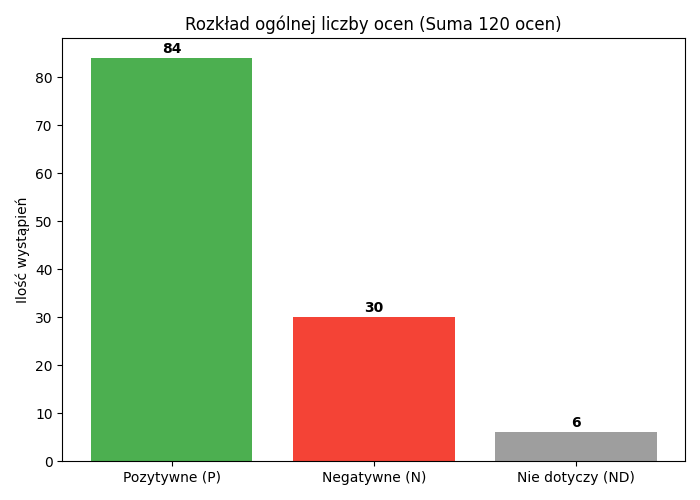
\includegraphics[width=0.94\linewidth]{chart_answers.png}

    \column{0.38\textwidth}
      \vspace{0.08cm}
      \statbox{statGreen}{84}{oceny pozytywne}
      \vspace{0.18cm}
      \statbox{statRed}{30}{ocen negatywnych}
      \vspace{0.18cm}
      \statbox{statBlue}{6}{ocen ``nie dotyczy''}

      \vspace{0.2cm}
      \small W praktyce oznacza to solidne podstawy dostępności, ale nie brak problemów.
  \end{columns}
\end{frame}

\begin{frame}{Zgodność audytorów}
  \begin{columns}[T,totalwidth=\textwidth]
    \column{0.55\textwidth}
      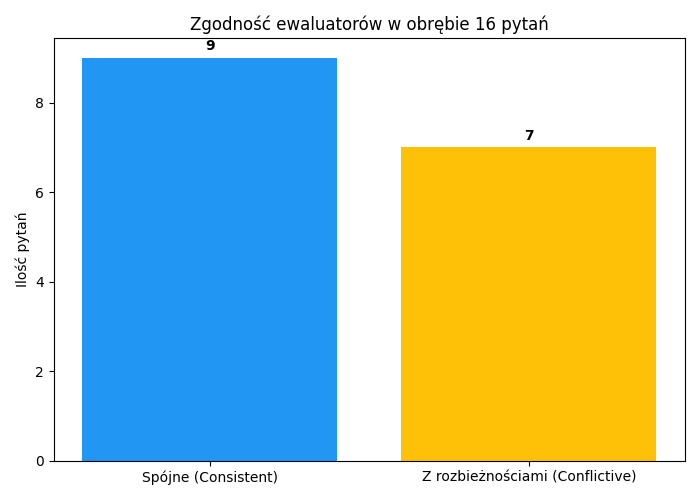
\includegraphics[width=0.94\linewidth]{chart_consistency.png}

    \column{0.38\textwidth}
      \vspace{0.05cm}
      \begin{block}{Interpretacja}
        \begin{itemize}
          \item \textbf{18} pytań: spójne w surowym zliczeniu.
          \item \textbf{12} pytań: z rozbieżnościami.
          \item \textbf{15} pytań: jednomyślnie pozytywne.
        \end{itemize}
      \end{block}

      \begin{alertblock}{Wniosek metodyczny}
        \footnotesize Raport wyróżnia też 6 kryteriów z co najmniej trzema ocenami negatywnymi albo pełną niezgodnością oraz 1 kryterium ND.
      \end{alertblock}
  \end{columns}
\end{frame}

\begin{frame}{Odpowiedzi na pytania Q1-Q2}
  \tagline{Wyniki z checklisty zostały przypisane do pytań badawczych, a nie tylko zliczone ogólnie.}

  \vspace{0.2cm}
  \small
  \begin{columns}[T,totalwidth=\textwidth]
    \column{0.48\textwidth}
      \begin{block}{Q1: obsługa wyłącznie klawiaturą}
        \textbf{Odpowiedź:} nie w pełni.

        \vspace{0.15cm}
        \begin{itemize}
          \item 2.1.1 Klawiatura: \textbf{4/4 P}
          \item 2.4.3 Kolejność fokusu: \textbf{4/4 P}
          \item 2.4.7 Widoczny fokus: \textbf{4/4 P}
          \item 2.1.2 Pułapki klawiaturowe: \textbf{2/4 N}
        \end{itemize}

        \vspace{0.1cm}
        \footnotesize Proces da się przejść, ale galerie i popupy wymagają lepszego zarządzania fokusem.
      \end{block}

    \column{0.48\textwidth}
      \begin{block}{Q2: interpretacja przez czytniki ekranu}
        \textbf{Odpowiedź:} częściowo.

        \vspace{0.15cm}
        \begin{itemize}
          \item standardowe \texttt{alt}: \textbf{4/4 P}
          \item złożone grafiki: \textbf{2 N, 1 P, 1 ND}
          \item nagłówki: \textbf{3/4 N}
          \item dynamiczne komponenty: \textbf{3/4 N}
          \item nowe karty bez ostrzeżenia: \textbf{4/4 N}
        \end{itemize}
      \end{block}
  \end{columns}
\end{frame}

\begin{frame}{Odpowiedzi na pytania Q3-Q4}
  \small
  \begin{columns}[T,totalwidth=\textwidth]
    \column{0.48\textwidth}
      \begin{block}{Q3: czytelność, powiększenie i formularze}
        \textbf{Odpowiedź:} raczej tak, ale z wyjątkami.

        \vspace{0.15cm}
        \begin{itemize}
          \item kontrast tekstu 4,5:1: \textbf{4/4 P}
          \item reflow i odstępy: \textbf{4/4 P}
          \item powiększenie 200\%: \textbf{3/4 P}
          \item tekst w obrazach: \textbf{4/4 N}
          \item identyfikacja błędów: \textbf{3/4 P}
        \end{itemize}

        \vspace{0.1cm}
        \footnotesize Najsłabsze miejsca to treści sprzedawców i komunikaty błędów poza fokusem.
      \end{block}

    \column{0.48\textwidth}
      \begin{block}{Q4: zbiorczy poziom dostępności}
        \textbf{Odpowiedź:} dobry, ale niepełny.

        \vspace{0.15cm}
        \begin{itemize}
          \item \textbf{84/120 P} = 70,0\% wszystkich ocen
          \item \textbf{84/114 P} = 73,7\% ocen aplikowalnych
          \item \textbf{18/30} pytań spójnych
          \item \textbf{12/30} pytań z rozbieżnościami
          \item \textbf{10} usterek: 6 istotnych, 4 nieistotne
        \end{itemize}
      \end{block}
  \end{columns}
\end{frame}

\begin{frame}{Co działało dobrze?}
  \tagline{Najważniejsze kroki procesu zakupowego były możliwe do przejścia w badanym zakresie.}

  \vspace{0.25cm}
  \begin{columns}[T,totalwidth=\textwidth]
    \column{0.47\textwidth}
      \begin{exampleblock}{Mocne strony}
        \begin{itemize}
          \item elementy aktywne w głównej ścieżce były dostępne klawiaturą,
          \item fokus był widoczny,
          \item kolejność fokusu była logiczna,
          \item kontrast tekstów w badanej ścieżce spełniał minimum.
        \end{itemize}
      \end{exampleblock}

    \column{0.47\textwidth}
      \begin{exampleblock}{Bezpieczne elementy procesu}
        \begin{itemize}
          \item brak automatycznie uruchamianego dźwięku,
          \item poprawne użycie większości elementów akcji,
          \item jasne etykiety przy kluczowych polach formularzy.
        \end{itemize}
      \end{exampleblock}
  \end{columns}
\end{frame}

\begin{frame}{Najważniejsze bariery}
  \small
  \renewcommand{\arraystretch}{1.22}
  \begin{tabularx}{\textwidth}{>{\bfseries}p{0.22\textwidth} Y p{0.21\textwidth}}
    \toprule
    Obszar & Problem & Grupa \\
    \midrule
    Galerie i popupy &
    Pułapki klawiaturowe po otwarciu powiększenia zdjęcia. &
    klawiatura / NVDA \\
    Filtry AJAX &
    Zmiana wyników bez jasnego komunikatu dla czytnika ekranu. &
    NVDA \\
    Opisy ofert &
    Problemy z tekstami alternatywnymi i hierarchią nagłówków. &
    niewidomi / słabowidzący \\
    \bottomrule
  \end{tabularx}

  \vspace{0.5cm}
  \normalsize
  \textcolor{RiskRed}{\textbf{W pełni negatywne kryteria:}}
  tekst w postaci obrazów oraz brak ostrzeżenia przed nową kartą.
\end{frame}

\begin{frame}{Pełna lista wykrytych błędów}
  \tagline{Po omówieniu najważniejszych przykładów warto pokazać, że raport zawierał pełną listę usterek i rekomendacji.}

  \vspace{0.2cm}
  \scriptsize
  \begin{columns}[T,totalwidth=\textwidth]
    \column{0.49\textwidth}
      \begin{enumerate}
        \item \textbf{Strona główna:} brak tekstów alternatywnych w grafikach promocyjnych.
        \item \textbf{Wyniki wyszukiwania:} dynamiczne przeładowanie filtrów nie jest anonsowane głosowo.
        \item \textbf{Szczegóły oferty:} zaburzona struktura nagłówków w opisach sprzedawców.
        \item \textbf{Galeria zdjęć:} możliwość uwięzienia fokusu w trybie pełnoekranowym.
        \item \textbf{Koszyk i dostawa:} błędy walidacji pojawiają się bez przeniesienia fokusu.
      \end{enumerate}

    \column{0.49\textwidth}
      \begin{enumerate}
        \setcounter{enumi}{5}
        \item \textbf{Stopka:} linki zewnętrzne otwierają nową kartę bez ostrzeżenia.
        \item \textbf{Wyniki 200\%:} ikonki dostawy mogą nakładać się na tekst.
        \item \textbf{Płatność:} przycisk finalizacji generuje powtórzenia w czytniku ekranu.
        \item \textbf{Opis oferty:} ważny tekst bywa osadzony w nieedytowalnych grafikach.
        \item \textbf{Formularz dostawy:} brak \texttt{autocomplete} dla danych zamawiającego.
      \end{enumerate}
  \end{columns}

  \vspace{0.25cm}
  \small
  \textcolor{RiskRed}{\textbf{Istotne:}} 1, 2, 4, 5, 6, 9
  \hfill
  \textcolor{Slate}{\textbf{Nieistotne:}} 3, 7, 8, 10
\end{frame}

\begin{frame}{Rekomendacje dla platformy}
  \tagline{Najpierw warto naprawiać bariery, które mogą zablokować wykonanie zadania.}

  \vspace{0.25cm}
  \begin{columns}[T,totalwidth=\textwidth]
    \column{0.48\textwidth}
      \begin{alertblock}{Priorytet wysoki}
        \begin{itemize}
          \item ujednolicić galerie i modale: obsługa \texttt{Esc}, zarządzanie fokusem,
          \item dodać regiony \texttt{aria-live} dla dynamicznie zmienianych wyników,
          \item kierować fokus na komunikaty błędów w koszyku i formularzach.
        \end{itemize}
      \end{alertblock}

    \column{0.48\textwidth}
      \begin{block}{Priorytet średni}
        \begin{itemize}
          \item wymuszać lepsze \texttt{alt} i nagłówki w szablonach sprzedawców,
          \item informować o linkach otwieranych w nowej karcie,
          \item dopracować układ przy powiększeniu 200\%.
        \end{itemize}
      \end{block}
  \end{columns}
\end{frame}

\begin{frame}{Wnioski końcowe}
  \begin{columns}[T,totalwidth=\textwidth]
    \column{0.48\textwidth}
      \begin{exampleblock}{Ocena ogólna}
        Allegro ma solidne podstawy dostępności w badanej ścieżce: wyszukiwanie, oferta i koszyk były możliwe do przejścia.

        \vspace{0.25cm}
        Nie oznacza to jednak pełnej dostępności. Znalezione bariery mogą obniżać komfort, a miejscami blokować użytkowników.
      \end{exampleblock}

    \column{0.48\textwidth}
      \begin{block}{Lessons learned}
        \begin{itemize}
          \item automatyczne narzędzia nie wystarczają bez testów manualnych,
          \item personalizowany e-commerce jest trudny do powtarzalnego audytu,
          \item w kolejnym badaniu warto użyć czystego profilu Chrome i jednakowej rozdzielczości,
          \item wyniki dotyczą badanej ścieżki, nie całego portalu.
        \end{itemize}
      \end{block}
  \end{columns}
\end{frame}

\end{document}
